\documentclass[10pt, compress]{beamer}

\usetheme[numbering=fraction, progressbar=frametitle]{metropolis}
\usepackage{booktabs}
\usepackage{array}
\usepackage{listings}
\usepackage{graphicx}
\usepackage[brazilian]{babel}
\usepackage[scale=2]{ccicons}
\usepackage{url}
\usepackage{relsize}
\usepackage{courier}
\usepackage{listings}
\usepackage{wasysym}

\usepackage{pgfplots}
\usepgfplotslibrary{dateplot}

\lstset{basicstyle=\footnotesize\ttfamily,breaklines=true}
\renewcommand*{\UrlFont}{\ttfamily\smaller\relax}

\graphicspath{{./img/}}

\title{INTRODUÇÃO À PROGRAMAÇÃO PARA GPUs USANDO CUDA}
\author{\footnotesize Pedro Bruel \\ {\scriptsize phrb@ime.usp.br}}
\institute{
\includegraphics[height=2cm]{imelogo}\\[0.2cm] Instituto de Matemática e Estatística \\ Universidade de São Paulo}
\date{\scriptsize 29 de Setembro de 2015}

\begin{document}

\maketitle

\begin{frame}
    \frametitle{ROTEIRO}
    \setbeamertemplate{section in toc}[sections numbered]
    \begin{enumerate}
        \item Introdução
            \begin{itemize}
                \item Recapitulando: Um \emph{template} para programas CUDA
                \item \emph{Profilers} e \emph{Debuggers}
            \end{itemize}
            \pause
        \item Ferramentas
            \begin{itemize}
                \item \texttt{nvcc}
                \item \texttt{nvprof}
                \item \texttt{cuda-gdb}
                \item \texttt{cuda-memcheck}
            \end{itemize}
    \end{enumerate}
\end{frame}

\begin{frame}
    \frametitle{RECURSOS}

    Os \emph{pdf}s com as aulas e todo o código fonte usado nos exemplos estão
    no \alert{GitHub}:

    \begin{itemize}
        \item \url{github.com/phrb/aulas-gpu}
    \end{itemize}
    \pause

    Outros recursos:

    \begin{itemize}
        \item CUDA Toolkit Documentation: \url{docs.nvidia.com/cuda}
        \item GPU Teaching Kit: \url{syllabus.gputeachingkit.com}
        \item iPython: \url{ipython.org/notebook.html}
        \item CUDA Toolkit: \url{developer.nvidia.com/cuda-toolkit}
        \item Anaconda: \url{continuum.io/downloads}
    \end{itemize}
\end{frame}

\begin{frame}[fragile]
    \frametitle{UM \textit{TEMPLATE} PARA CUDA C}
    \begin{lstlisting}[basicstyle=\scriptsize, language=C]
    // Código em src/cuda-samples/0_Simple/vectorAdd/vectorAdd.cu
    #include <cuda_runtime.h>
    \end{lstlisting}
    \pause
    \begin{lstlisting}[basicstyle=\scriptsize, language=C]
    float *h_A = (float *)malloc(size);
    if (h_A == NULL) { ... };

    err = cudaMalloc((void **)&d_A, size);
    err = cudaMemcpy(d_A, h_A, size, cudaMemcpyHostToDevice);
    if (err != cudaSuccess) { ... };
    \end{lstlisting}
    \pause
    \begin{lstlisting}[basicstyle=\scriptsize, language=C]
    int threadsPerBlock = 256;
    int blocksPerGrid =(numElements + threadsPerBlock - 1) / threadsPerBlock;
    \end{lstlisting}
    \pause
    \begin{lstlisting}[basicstyle=\scriptsize, language=C]
    vectorAdd<<<blocksPerGrid, threadsPerBlock>>>(d_A, d_B, d_C, numElements);

    err = cudaGetLastError()
    err = cudaDeviceSynchronize()
    if (err != cudaSuccess) { ... };
    \end{lstlisting}
    \pause
    \begin{lstlisting}[basicstyle=\scriptsize, language=C]
    err = cudaMemcpy(h_C, d_C, size, cudaMemcpyDeviceToHost);
    err = cudaFree(d_A);
    if (err != cudaSuccess) { ... };
    \end{lstlisting}
\end{frame}

\begin{frame}
    \frametitle{UM \textit{TEMPLATE} PARA CUDA C}
    Exemplos no repositório:
    \small
    \begin{itemize}
        \item \texttt{src/cuda-samples/0\_Simple}
        \item \texttt{src/cuda-samples/0\_Simple/vectorAdd/vectorAdd.cu}
        \item \texttt{src/cuda-samples/0\_Simple/template\_runtime/template\_runtime.cu}
    \end{itemize}
\end{frame}

\begin{frame}
    \frametitle{\textit{PROFILERS} E \textit{DEBUGGERS}}
    \textit{Profilers}:
    \begin{itemize}
        \item Ferramentas para análise de código \alert{em tempo de execução}
        \item A intenção é \alert{otimizar o código}
    \end{itemize}
    \pause
    Como?
    \begin{itemize}
        \item Instrumentação do Código
        \item Captura de eventos
        \item Geração de dados
    \end{itemize}
    \pause
    O quê?
    \begin{itemize}
        \item Consumo de memória
        \item Frequência e duração de chamadas de função
        \item Uso de instruções específicas
        \pause
        \item \alert{Bottlenecks}, ou \alert{Gargalos}, de desempenho
    \end{itemize}
\end{frame}

\begin{frame}
    \frametitle{\textit{PROFILERS} E \textit{DEBUGGERS}}
    \textit{Debuggers}:
    \begin{itemize}
        \item Ferramentas para análise de código \alert{em tempo de execução}
        \item As intenções são \alert{consertar bugs} e realizar \alert{testes}
    \end{itemize}
    \pause
    Como?
    \begin{itemize}
        \item Instrumentação do Código
        \item Execução passo-a-passo
        \item \alert{Breakpoints}
    \end{itemize}
    \pause
    O quê?
    \begin{itemize}
        \item Acessos e vazamentos de memória
        \item Pode ajudar com vários tipos de \alert{bugs} \smiley{}
    \end{itemize}
\end{frame}

\begin{frame}
    \frametitle{RECURSOS}
    Os próximos \emph{slides} foram adaptados do
    material disponível no \alert{GPU Teaching Kit}:
    \begin{itemize}
        \item \url{syllabus.gputeachingkit.com}
    \end{itemize}
\end{frame}

\begin{frame}
    \begin{figure}[H]
        \centering
        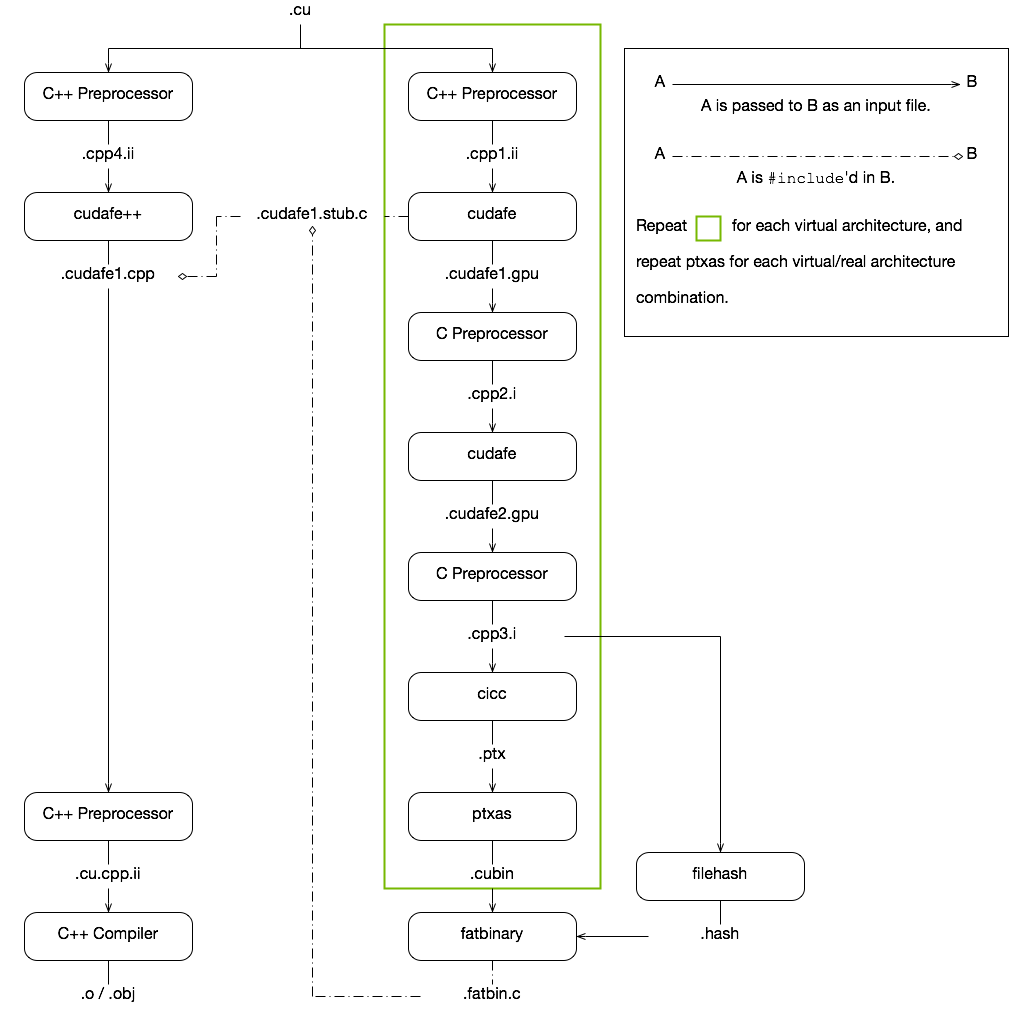
\includegraphics[width=.8\textwidth]{cuda-compilation}
    \end{figure}
\end{frame}

\plain{Obrigado!}

\maketitle

\end{document}
